\pagestyle{empty}
\centering
\fontsize{2cm}{2cm}\selectfont{System Design Document} \\
\vspace{2mm}
\fontsize{1cm}{1cm}\selectfont Audio digital signal processor \\
\vspace{2mm}
\large BeCreative Minor\\
\normalsize
\vspace{4cm}
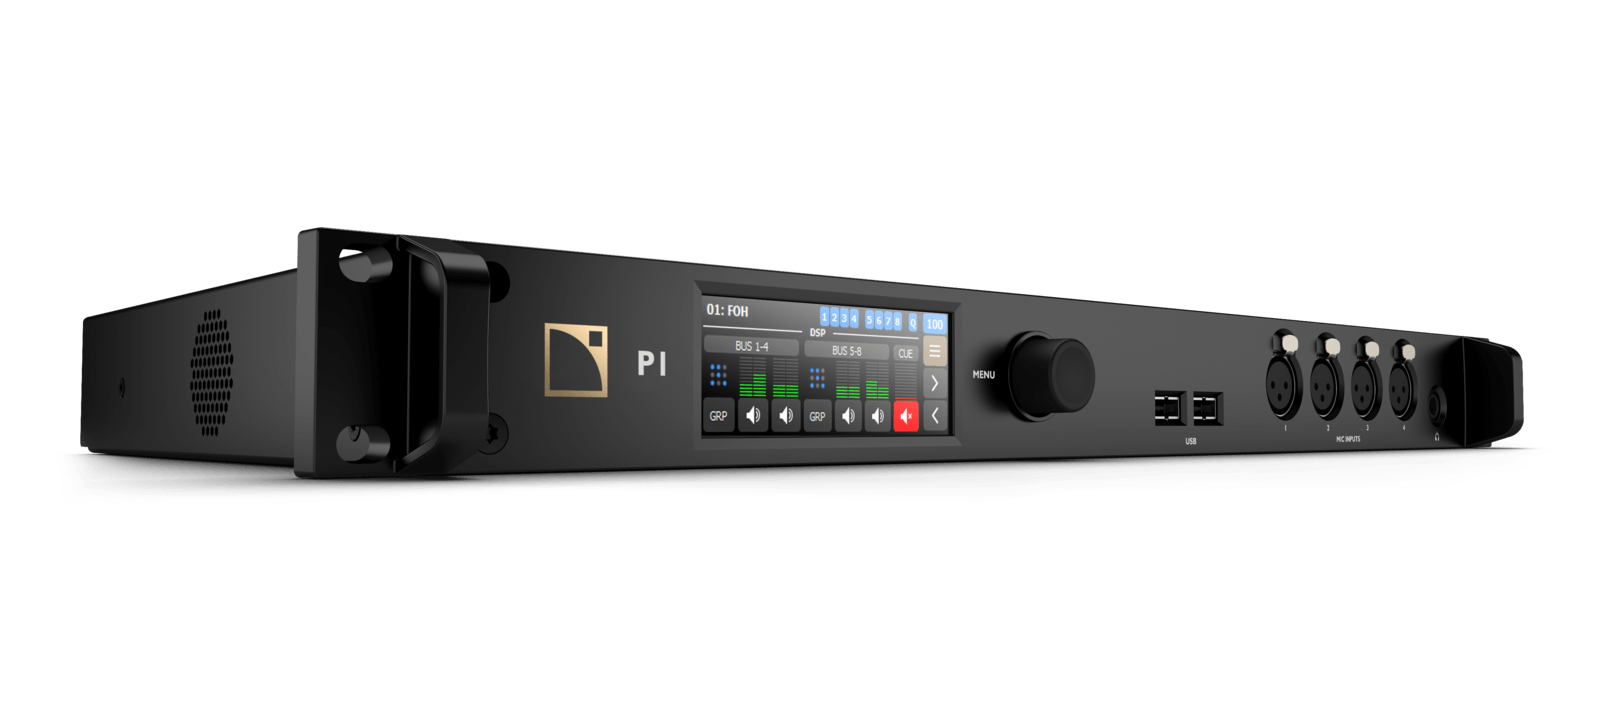
\includegraphics[width=\linewidth]{3DR_P1_Perspective.png}\\
\vfill
\normalsize Busse Lommers \\
Robin van den Dungen \\
Mahmud Gürler \\
Silas Kamphuis \\
Hein Verhallen \\
Youri Tils \\
Ahmed Abdelrahim \\
Fontys Hogescholen, De Rondom 1, 5612 AP Eindhoven \\
\today

\begin{justify}


\newpage
\tableofcontents
\thispagestyle{empty}

\listoffigures
\thispagestyle{empty}

\listoftables
\thispagestyle{empty}

\newpage
\pagestyle{plain}
\setcounter{page}{1}

\chapter*{Abbreviation List}

\begin{table}[!h]
	\centering
\begin{tabular}{|c|c|}
	\hline
\textbf{Abbreviation} & \textbf{Explanation}        \\ \hline
<<<<<<< Updated upstream
ADC                   & Analog to Digital Converter  \\ \hline
DAC                   & Digital to Analog Converter \\ \hline
DSP                   & Digital Signal Processor \\ \hline
FPGA				  & Field-Programmable Gate Array \\ \hline
Hi-Fi                 & High Fidelity \\ \hline
IC        	       	  & Integrated Circuit \\ \hline
LDO					  & Low DropOut \\ \hline
SEPIC				  & Single-Ended Primary-Inductor
Converter \\ \hline
UI					  & User Interface \\ \hline
=======
DSP                  & Digital Signal Processor \\ \hline
DAC                  & Digital-to-Analog Converter \\ \hline
ADC	                 & Analog-to-Digital Converter \\ \hline
>>>>>>> Stashed changes
\end{tabular}
\caption{List of commonly used Abbreviations}
\label{Abbreviation list}
\end{table}